\documentclass[conference]{IEEEtran}
\IEEEoverridecommandlockouts
\usepackage{amsmath}
\usepackage{newtxtext,newtxmath}
\usepackage{graphicx}
\usepackage{booktabs}
\usepackage{tikz}
\usetikzlibrary{arrows.meta,positioning}
\usepackage[hidelinks]{hyperref}
\usepackage{cite}

\begin{document}

\title{Catching RAG Hallucinations from Inside the Model: Reproducing and Stress-Testing ReDeEP}

\author{\IEEEauthorblockN{Adithya K}
\IEEEauthorblockA{Deep Learning Course Project, Semester VII\\
October 2026}}

\maketitle

\begin{abstract}
We reproduce ReDeEP, a mechanistic-interpretability method for detecting hallucinations in retrieval-augmented generation (RAG), on the RAGTruth benchmark using a single 6\,GB laptop GPU. On the paper's own backbone, Llama-2-7B-chat, our detector reaches an AUC of 0.739 against the published 0.7325. Across four LLaMA-family models from 1.1B to 7B parameters, ReDeEP outperforms perplexity and length-normalised entropy baselines by 0.06 to 0.11 AUC. We then stress-test the method: replacing the retrieved passage with an irrelevant one raises the hallucination score sharply, but corrupting the passage's numbers, so that the response contradicts it, leaves the score unchanged or even lowers it. ReDeEP therefore measures whether a response is \emph{about} its context, not whether it \emph{agrees} with it. Finally, prompted black-box judges from the Gemini and GPT families (AUC 0.827 and 0.790) outperform ReDeEP (0.721) on the same held-out responses, while a small 3B LLaMA judge performs at chance (0.499).
\end{abstract}

\begin{IEEEkeywords}
hallucination detection, retrieval-augmented generation, mechanistic interpretability, large language models, robustness
\end{IEEEkeywords}

\section{Introduction}
Retrieval-augmented generation grounds a language model's answer in a retrieved passage, yet models still produce claims that the passage does not support. Such RAG hallucinations are difficult to catch with output-only signals such as perplexity, because a fluent, confident answer can still ignore its context.

ReDeEP~\cite{sun2025redeep} explains RAG hallucinations mechanistically. \emph{Copying heads}---attention heads that move context tokens into the residual stream---carry external knowledge, while \emph{knowledge FFNs}---feed-forward layers---inject the model's parametric knowledge. A hallucination occurs when the model under-uses the former and over-relies on the latter. ReDeEP converts both into scores and regresses the hallucination label on them.

This project makes three contributions:
\begin{enumerate}
\item A faithful reproduction of ReDeEP's token-level detector on RAGTruth~\cite{niu2024ragtruth} on consumer hardware (RTX~4050, 6\,GB VRAM), including memory optimisations that make 7B models feasible.
\item A transfer study across four LLaMA-family backbones~\cite{touvron2023llama2} from 1.1B to 7B parameters.
\item An extension that stress-tests ReDeEP under corrupted retrieval, and a comparison against black-box LLM judges from the GPT, Gemini and LLaMA families.
\end{enumerate}

\section{Method}
\begin{figure}[t]
\centering
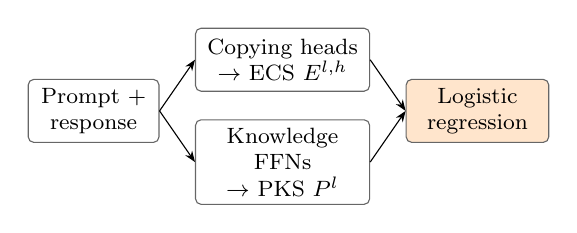
\begin{tikzpicture}[font=\footnotesize, box/.style={draw=black!60, rounded corners=2pt, align=center, minimum height=8mm, inner sep=3pt}, >={Stealth[length=4pt]}]
\node[box, text width=1.45cm] (in) {Prompt +\\response};
\node[box, text width=2.0cm, right=0.45cm of in, yshift=6.5mm] (ecs) {Copying heads\\$\rightarrow$ ECS $E^{l,h}$};
\node[box, text width=2.0cm, right=0.45cm of in, yshift=-6.5mm] (pks) {Knowledge FFNs\\$\rightarrow$ PKS $P^{l}$};
\node[box, text width=1.6cm, right=0.45cm of ecs, yshift=-6.5mm, fill=orange!20] (out) {Logistic\\regression};
\draw[->] (in.east) -- (ecs.west); \draw[->] (in.east) -- (pks.west);
\draw[->] (ecs.east) -- (out.west); \draw[->] (pks.east) -- (out.west);
\end{tikzpicture}
\caption{ReDeEP pipeline: one forward pass yields an external-context score per head and a parametric-knowledge score per FFN layer; a logistic regression combines them into a hallucination score.}
\label{fig:pipeline}
\end{figure}

Fig.~\ref{fig:pipeline} summarises the detector. All quantities are computed from a single forward pass over the prompt (instruction and retrieved passage) followed by the response; $R$ denotes the set of response token positions.

\subsection{External Context Score}
For head $h$ in layer $l$ and response token $n$, let $\mathcal{T}_n$ be the 10\% of context tokens the head attends to most. With $x^{L}_i$ the final-layer hidden state of token $i$,
\begin{equation}
E^{l,h} = \frac{1}{|R|}\sum_{n\in R}\cos\!\Big(\tfrac{1}{|\mathcal{T}_n|}\textstyle\sum_{i\in\mathcal{T}_n} x^{L}_{i},\; x^{L}_{n}\Big).
\end{equation}
A high ECS means the response is built from what the head read in the context.

\subsection{Parametric Knowledge Score}
For layer $l$, the residual stream just before ($x^{\mathrm{mid},l}$) and after ($x^{l}$) the FFN block is projected to the vocabulary with the LogitLens~\cite{logitlens}:
\begin{equation}
P^{l} = \frac{1}{|R|}\sum_{n\in R}\mathrm{JSD}\big(p^{\mathrm{mid},l}_n,\; p^{l}_n\big),
\end{equation}
where $p_n = \sigma(W_U\,\mathrm{norm}(x_n))$ is the LogitLens next-token distribution of a residual state, $\sigma$ the softmax and JSD the Jensen--Shannon divergence. A large shift indicates that the FFN injected its own knowledge.

\subsection{Detector and Baselines}
Copying heads are ranked by their OV circuit, scored on 500 sampled vocabulary tokens (large trace, few Gershgorin-disc outliers); the top 8 form set $\mathcal{A}$. On each training fold, the 5 layers whose PKS correlates most positively with the label form set $\mathcal{F}$. A logistic regression is fitted on the standardised features $\bar{P}_{\mathcal{F}}$ and $-\bar{E}_{\mathcal{A}}$, with the decision threshold set at the best-F1 point on the training fold. Baselines are the response perplexity and LN-Entropy~\cite{malinin2021uncertainty} (mean per-token predictive entropy) from the same forward pass.

\subsection{Black-Box Judges}
Each judge receives the RAG input and the response and must reply in JSON with the probability (0--100) that the response contains a claim the passage contradicts or does not support, judging against the passage only. The stated probability is used as the score.

\section{Experimental Setup}
All models score the same 415 responses: the RAGTruth test split restricted to responses generated by llama-2-7b-chat, the paper's setting, capped at 6{,}000 characters; 212 are hallucinated. Table~\ref{tab:backbones} lists the backbones.

\begin{table}[t]
\caption{Backbones (ungated Hugging Face mirrors with identical weights)}
\label{tab:backbones}
\centering\footnotesize
\begin{tabular}{@{}lll@{}}
\toprule
Backbone & Params & Precision \\
\midrule
TinyLlama-1.1B-Chat & 1.1B & fp16 \\
Llama-3.2-1B-Instruct & 1.2B & fp16 \\
Llama-3.2-3B-Instruct & 3.2B & 4-bit NF4 \\
Llama-2-7B-chat & 6.7B & 4-bit NF4 \\
\bottomrule
\end{tabular}
\end{table}

Experiments ran on a Lenovo LOQ laptop (RTX~4050, 6\,GB VRAM, 16\,GB RAM) with PyTorch~2.11, transformers~5.17 and bitsandbytes~0.50. Sequences are capped at 1{,}024 tokens, truncating the prompt from the left so that the whole response is scored. We report the mean and standard deviation over stratified 5-fold cross-validation; heads and layers are re-selected inside each training fold, so no test labels leak into selection.

\textbf{Engineering for 6\,GB.} The reference implementation requests every full attention map, which does not fit for 7B models. We replaced it with forward hooks that keep only each layer's top-$k$ context indices, and compute the attended mean as a sparse matrix product. On a RAGTruth example the rewritten ECS matches the original to within $6\times10^{-8}$. Scoring takes about 0.6\,s per example for TinyLlama and 4--7\,s for Llama-2-7B.

\section{Results}
\subsection{Hallucination Detection}
\begin{figure}[t]
\centering
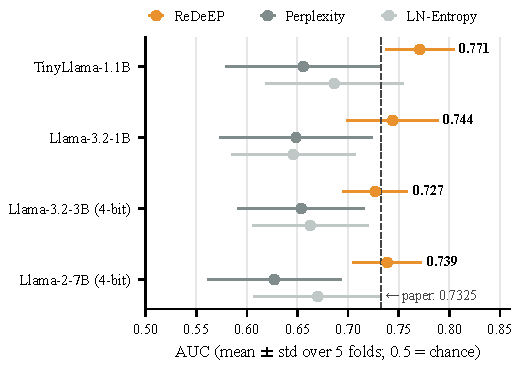
\includegraphics[width=\columnwidth]{figures/detection_auc.pdf}
\caption{Detection AUC per backbone. ReDeEP (orange) beats both baselines on every model; the dashed line marks the paper's Llama-2-7B result.}
\label{fig:detection}
\end{figure}

\begin{table}[t]
\caption{Detection results, 5-fold CV mean ($n=415$)}
\label{tab:detection}
\centering\footnotesize
\setlength{\tabcolsep}{3.5pt}
\begin{tabular}{@{}lccccc@{}}
\toprule
& \multicolumn{3}{c}{ReDeEP} & PPL & LN-Ent \\
\cmidrule(lr){2-4}
Backbone & AUC & PCC & F1 & AUC & AUC \\
\midrule
TinyLlama-1.1B & \textbf{0.771} & 0.475 & 0.718 & 0.656 & 0.686 \\
Llama-3.2-1B & \textbf{0.744} & 0.426 & 0.692 & 0.649 & 0.646 \\
Llama-3.2-3B (4-bit) & \textbf{0.727} & 0.399 & 0.695 & 0.654 & 0.663 \\
Llama-2-7B (4-bit) & \textbf{0.739} & 0.427 & 0.687 & 0.627 & 0.670 \\
\midrule
Paper (Llama-2-7B) & 0.7325 & 0.3979 & -- & -- & -- \\
\bottomrule
\end{tabular}
\end{table}

ReDeEP reproduces on the paper's backbone: Llama-2-7B reaches an AUC of 0.739 ($\pm$0.034) against the published 0.7325, and a PCC of 0.427 against 0.3979 (Table~\ref{tab:detection}, Fig.~\ref{fig:detection}). ReDeEP beats both baselines on every backbone, by 0.06 (Llama-3.2-3B, vs.\ LN-Entropy) to 0.10 (Llama-3.2-1B, vs.\ perplexity) over the better baseline. Detection quality is roughly flat in model size: the 1.1B TinyLlama scores highest, and the 3B and 7B models lie within one standard deviation of each other. The baselines also vary more across folds (std 0.06--0.08) than ReDeEP does (0.03--0.05).

\subsection{Black-Box LLM Judges}
\begin{figure}[t]
\centering
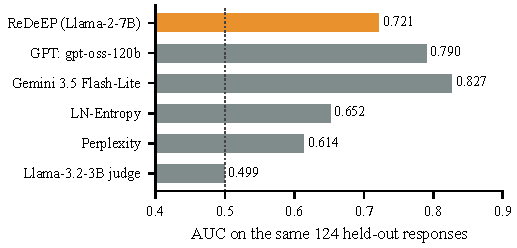
\includegraphics[width=\columnwidth]{figures/judges_auc.pdf}
\caption{All detectors on the same 124 held-out responses. The API judges are more accurate; a small local judge is at chance.}
\label{fig:judges}
\end{figure}

\begin{table}[t]
\caption{Judges vs.\ ReDeEP on the same 124 held-out responses}
\label{tab:judges}
\centering\footnotesize
\setlength{\tabcolsep}{3pt}
\begin{tabular}{@{}llcccc@{}}
\toprule
Detector & Kind & AUC & PCC & Rec. & F1 \\
\midrule
Gemini 3.5 Flash-Lite & Judge & \textbf{0.827} & 0.671 & 0.914 & 0.865 \\
GPT: gpt-oss-120b & Judge & 0.790 & 0.465 & 0.929 & 0.778 \\
ReDeEP (Llama-2-7B) & Internals & 0.721 & 0.390 & 0.714 & 0.714 \\
LN-Entropy & Uncertainty & 0.652 & -- & -- & -- \\
Perplexity & Uncertainty & 0.614 & -- & -- & -- \\
Llama-3.2-3B (local) & Judge & 0.499 & -0.005 & 0.071 & 0.127 \\
\bottomrule
\end{tabular}
\end{table}

Large prompted judges outperform ReDeEP (Table~\ref{tab:judges}, Fig.~\ref{fig:judges}): Gemini 3.5 Flash-Lite reaches 0.827 and OpenAI's open-weights gpt-oss-120b~0.790, against 0.721 for ReDeEP on the same 124 responses. On all 415 responses the Gemini judge scores 0.810, consistent with the held-out result. Because the judges read the passage and the response as text, they can spot a contradicted fact directly---exactly ReDeEP's blind spot (Section~\ref{sec:robust}). A small prompted judge fails: Llama-3.2-3B answers ``no hallucination'' almost always (AUC 0.499), whereas reading the internals of a model of the same size (ReDeEP on Llama-3.2-3B, AUC 0.727) works far better. ReDeEP's advantage is cost and access: one forward pass of a small open model, with no API, no per-call cost and no data leaving the machine.

\section{Extension: Robustness Under Corrupted Retrieval}
\label{sec:robust}
We hold each response fixed and change only the retrieved passage: (i) \emph{accurate}, the real passage; (ii) \emph{irrelevant}, a passage from a different source of the same task type; (iii) \emph{numbers corrupted}, every number in the real passage multiplied by a random factor in $[1.3, 3.0]$, so that numbers the response copied are now contradicted. The detector is refitted on the remaining 265 examples, so all 150 perturbed responses are held out.

\begin{figure}[t]
\centering
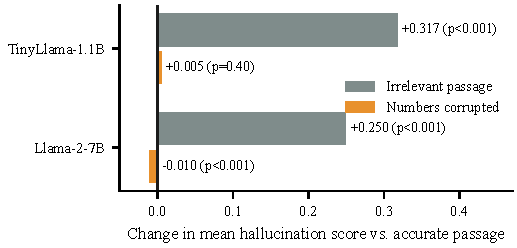
\includegraphics[width=\columnwidth]{figures/robustness_shift.pdf}
\caption{Change in mean ReDeEP score relative to the accurate passage (paired Wilcoxon test, 150 responses per backbone).}
\label{fig:robust}
\end{figure}

\begin{table}[t]
\caption{Robustness: mean score and signals per condition}
\label{tab:robust}
\centering\footnotesize
\setlength{\tabcolsep}{3pt}
\begin{tabular}{@{}llcccc@{}}
\toprule
Backbone & Condition & Score & ECS & PKS & AUC \\
\midrule
TinyLlama & Accurate & 0.522 & 0.326 & 0.158 & 0.755 \\
TinyLlama & Irrelevant & 0.840 & 0.244 & 0.187 & 0.545 \\
TinyLlama & Numbers corr. & 0.528 & 0.330 & 0.160 & 0.747 \\
\midrule
Llama-2-7B & Accurate & 0.521 & 0.282 & 0.091 & 0.710 \\
Llama-2-7B & Irrelevant & 0.770 & 0.288 & 0.114 & 0.564 \\
Llama-2-7B & Numbers corr. & 0.510 & 0.310 & 0.092 & 0.715 \\
\bottomrule
\end{tabular}
\end{table}

\textbf{Irrelevant passages work as intended.} The score jumps for nearly every response (+0.317 for TinyLlama, +0.250 for Llama-2-7B, both $p<0.001$), so the original labels stop separating the responses (AUC $\approx$0.55; Fig.~\ref{fig:robust}, Table~\ref{tab:robust}). This is correct behaviour, because nothing in the response is supported by the new passage. The mechanism differs by size: in TinyLlama ECS falls (0.326 to 0.244), whereas in Llama-2-7B ECS is flat and the increase comes from PKS (0.091 to 0.114).

\textbf{Corrupted numbers go unnoticed.} For TinyLlama the score does not move (+0.005, $p=0.40$). For Llama-2-7B it falls slightly (-0.010, $p<0.001$) while ECS rises (0.282 to 0.310): the detector rates a contradicted response as \emph{more} faithful. Restricted to the 122 responses that state a number the corrupted passage now contradicts, the score rose in only 52\% of cases for TinyLlama and 31\% for Llama-2-7B.

\textbf{Interpretation.} ECS is a cosine similarity between hidden states: it measures whether the response is built from what the copying heads read, not whether the facts match. A plausible explanation is that a changed number barely moves the hidden state, so ReDeEP cannot see it. The method thus catches topical hallucinations but needs a complementary fact-level check for numeric or entity contradictions.

\section{Limitations}
\begin{itemize}
\item \emph{Quantisation:} the 3B and 7B models ran in 4-bit NF4, so their ECS and PKS approximate full precision; the 7B match with the paper suggests the effect is small.
\item \emph{Sampled copying-head scores:} OV circuits are scored on 500 sampled vocabulary tokens rather than the full vocabulary.
\item \emph{One generator:} all responses come from llama-2-7b-chat, so the other backbones score text they did not write.
\item \emph{Sample size:} fold standard deviations are 0.03--0.05 AUC; smaller differences are within noise.
\item \emph{Robustness scope:} only numbers are corrupted; entity swaps and negations are untested.
\item \emph{Judge access:} judges ran on free API tiers; the GPT-family judge is the open-weights gpt-oss-120b, evaluated on the 124 held-out responses because of rate limits.
\end{itemize}

\section{Conclusion}
ReDeEP reproduces on a laptop GPU (AUC 0.739 vs.\ 0.7325) and beats uncertainty baselines on four LLaMA models from 1.1B to 7B parameters. Its signals catch responses that are off-topic for their context but not responses that contradict their context's numbers. Large prompted judges are more accurate but require an API; small prompted judges do not work. ReDeEP is therefore best used as a cheap, private first-line detector for topical hallucinations, paired with a fact-level check. Future work: entity and negation corruptions, a numeric-consistency feature combined with ECS, full-precision runs on larger GPUs with backbone-matched responses, and judge evaluation on all responses with repeated sampling.

\begin{thebibliography}{9}
\bibitem{sun2025redeep} Z.~Sun \emph{et al.}, ``ReDeEP: Detecting hallucination in retrieval-augmented generation via mechanistic interpretability,'' in \emph{Proc. Int. Conf. Learning Representations (ICLR)}, 2025.
\bibitem{niu2024ragtruth} C.~Niu \emph{et al.}, ``RAGTruth: A hallucination corpus for developing trustworthy retrieval-augmented language models,'' in \emph{Proc. Annu. Meeting Assoc. Comput. Linguistics (ACL)}, 2024.
\bibitem{touvron2023llama2} H.~Touvron \emph{et al.}, ``Llama 2: Open foundation and fine-tuned chat models,'' arXiv:2307.09288, 2023.
\bibitem{malinin2021uncertainty} A.~Malinin and M.~Gales, ``Uncertainty estimation in autoregressive structured prediction,'' in \emph{Proc. ICLR}, 2021.
\bibitem{logitlens} nostalgebraist, ``Interpreting GPT: the logit lens,'' LessWrong, 2020.
\end{thebibliography}

\end{document}
